% A simple template for LaTeX documents
% 
% To produce pdf run:
%   $ pdflatex paper.tex 
%

\documentclass[12pt]{article}

% Begin paragraphs with new line
\usepackage{parskip}  

% Change margin size
\usepackage[margin=1in]{geometry}   

% Graphics Example:  (PDF's make for good plots)
\usepackage{graphicx}               
% \centerline{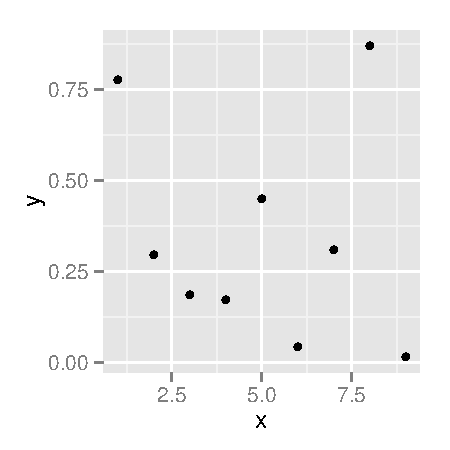
\includegraphics{figure.pdf}}

% Allows hyperlinks
\usepackage{hyperref}

% Blocks of code
\usepackage{listings}
\lstset{basicstyle=\ttfamily, title=\lstname}
% Insert code like this. replace `plot.R` with file name.
% \lstinputlisting{plot.R}

% Supports proof environment
\usepackage{amsthm}

% Allows writing \implies and align*
\usepackage{amsmath}

% Allows mathbb{R}
\usepackage{amsfonts}

% Allows alpha labels rather than numeric
\usepackage{enumitem}


%%%%%%%%%%%%%%%%%%%%%%%%%%%%%%%%%%%%%%%%%%%%%%%%%%%%%%%%%%%%

\begin{document}

\begin{center}
    {\Large Homework 1}\\
    \bigskip
    \bigskip
    \hrule
    \medskip
    Clark Fitzgerald\\
    Stats 206
\end{center}

\subsection*{2. True / False}
\begin{enumerate}[label=\alph*]
\item  \textbf{True} The least squares line always passes the center of the data.
This is implied by the calculation for $\hat{\beta_0} = \bar{Y} -
\hat{\beta_1} \bar{X}$.
The large point in the below plot is the center of the data.

\centerline{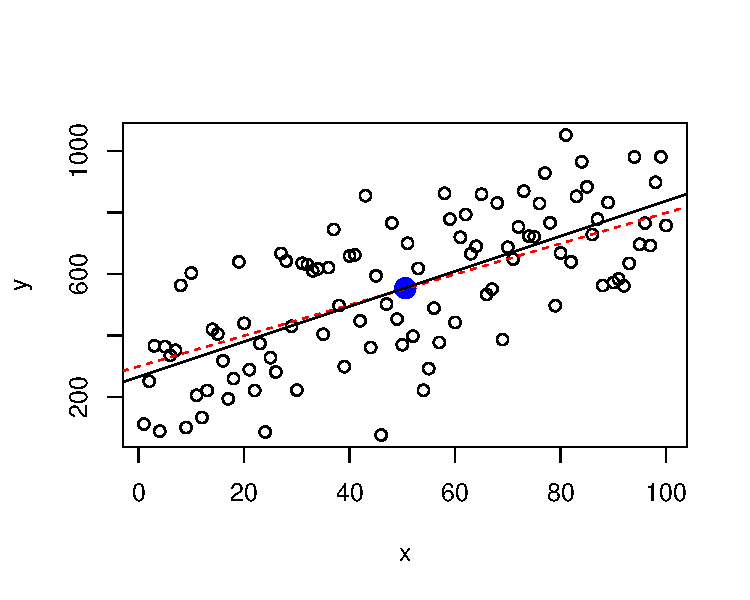
\includegraphics{regress.pdf}}

\item \textbf{False} The least squares line fits the data
best by definition. In the figure above the fitted regression line is the solid line,
while the true regression line is the dashed line. They are not the same.
\end{enumerate}

\end{document}
